\chapter{Literature Review}
% -_____________________________________________________________________________

This section introduces the basics of Ethereum and blockchains to the reader before acquainting them with the current state of research in the field.

% -_____________________________________________________________________________

\section{Blockchain Basics}

Blockchain technology has been acknowledged as a transformative innovation in many industries beyond cryptocurrencies, such as Internet of Things (IoT), healthcare and especially logistics and finance, since its inception in 2008 by Nakamoto in Bitcoin \cite{NakamotoBitcoin:System}. Compared to traditional centralised systems, blockchain offers several distinct advantages, including immutability, heightened security, fault tolerance, transparency and empowering users with a greater level of control through decentralisation.

\subsection{How it works}

Similar to a linked list, a blockchain is a series of 'blocks' containing some information, with each block linked to the block before, using deterministic cryptographic hashes. This forms an immutable chain of blocks holding hashed information that cannot be altered, known as the ledger, shown in \fref{Figure:BasicBlockchain}. Going back and altering any block in this ledger invalidates the hashes of all the blocks after it. This is what makes blockchains resistant to data modification (\textbf{immutable}). Each participating machine is called a node on the network. Each node holds its personal copy of the transactions and hashed blocks and is responsible for spreading any new transaction information to the whole network.

\begin{figure}[h]
    \centering
    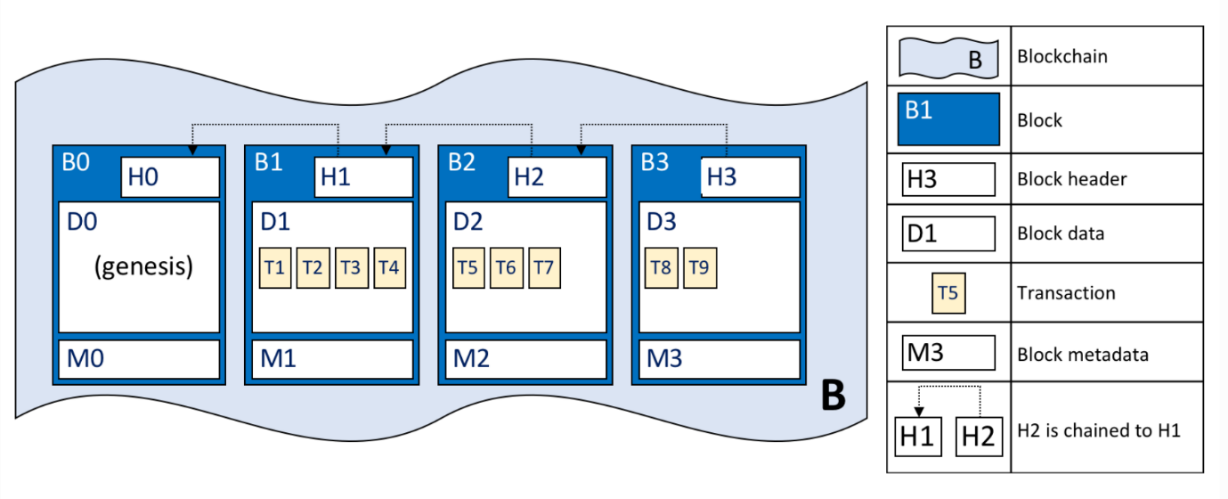
\includegraphics[width=13cm,center]{Figures/BlockchainStructure.png}
    \caption{The data structure underlying blockchain \cite{ADocumentation}. The first block is called the Genesis Block.}
    \label{Figure:BasicBlockchain}
\end{figure}

Blockchain removes the need for an intermediary, such as a bank, to mediate a transaction between 2 parties. External authorities are not required to validate the authenticity and integrity of data. It is a decentralised data structure that serves as the single source of truth to all nodes on the network creating trust between anonymous actors.



% -_____________________________________________________________________________

\subsection{Consensus Protocols}

The consensus protocol chosen determines how nodes validate and agree on any new transactions being added to the public ledger, and it varies between different blockchains. It makes sure that all nodes in a network have a consistent view of the ledger. This mechanism plays a crucial role in safeguarding against a variety of attacks that malicious nodes could attempt.
% -_____________________________________________________________________________

\subsubsection{Proof-Of-Work}

PoW is the consensus algorithm that couples voting weight with computing 
power. Thus it relies on computational resources to defend against the Sybil attack \cite{Sedlmeir2020TheMyth}.

\textbf{Miners} are nodes actively participating in the consensus-forming process. Miners compete 
to solve a computationally challenging mathematical puzzle in order to verify a group of transactions included in a block. In a brute-force manner, miners try to guess the right 'nonce' (number only used once) that when it is combined with the rest of the block header information and hashed, the hash has to have a certain number of leading zeros at the beginning. It is like trying to guess the number of a winning lottery ticket. It is challenging to produce (in terms of time and compute power) but easy to verify for other nodes \cite{Centieiro2021BitcoinCoding}. Once a node guesses the correct 'nonce', it broadcasts it to the rest of the network for validation. When most other miners have agreed on its legitimacy, the new block can permanently be added to the blockchain ledger, and the block proposer is rewarded with mining fees.

% -_____________________________________________________________________________

\subsubsection{Proof-Of-Stake}

PoS is a consensus protocol that relies on economic power rather than computational power to secure the network. It requires nodes called ‘validators’ to put up a set amount of their cryptocurrency at stake (as collateral). In exchange, they increase their chance of being randomly selected as the block proposer for the next round of transactions and consequently earn the block rewards that come with it \cite{King2012PPCoin:Proof-of-Stake}. In some implementations of PoW, the more a validator puts at stake, the higher their chance of being picked as the block proposer. If a validator submits a fraudulent transaction or tampers with transaction information, they risk losing their staked cryptocurrency and any block rewards they may have received, as other observing nodes always verify each new block \cite{Napoletano2022WhatAdvisor}. 

PoS is a much less energy-intensive design compared to PoW.

% -_____________________________________________________________________________

% -_____________________________________________________________________________

\section{Ethereum Basics}

Ethereum was introduced in 2015 by Vitalik Buterin as a blockchain platform with capabilities beyond cryptocurrency. It features smart contracts, which are segments of code that contain specific conditions. These contracts enable the creation of self-executing programs that activate automatically when the specified criteria are met. Ethereum's blockchain forms the backbone for a variety of applications, including Decentralized Applications (DApps), thanks to the functionality of smart contracts.

Nodes that communicate over a network following the 'ETH' protocol form the Ethereum network, also called the Ethereum 'mainnet'. These nodes contribute to maintaining and securing a globally agreed state of the Ethereum Virtual Machine (EVM). This was also described as 'one computer for the entire planet" by Ethereum co-founder Gavin Wood in 2016\cite{Ethereum:Industries}. 

The security of this network comes from a majority of nodes agreeing on the new change to the state of this EVM. In other words, agreeing on the next block to be permanently added to the blockchain ledger. Such nodes are paid in Ethereum's native cryptocurrency, \textbf{Ether (ETH)}, to run validator software that validates new blocks received over the peer-to-peer network.

***Introduce the need for consensus protocols

Ethereum is a public, permissionless network, which means that anyone can access and participate in its operations. The interaction between a client and the Ethereum blockchain is enabled by the JSON RPC(Remote Procedure Call) API. When any user wants to complete a transaction with another user across the network, they:
\begin{enumerate}
    \item Need to specify the transaction amount
    \item Secure the transaction with their own private key
    \item Specify the tip they are willing to pay on top of the base transaction fees (both in 'gas' units) to incentivise a validator to validate and include their transaction in an upcoming block
\end{enumerate}

The ETH Execution client verifies the transaction request by checking things like whether the user has enough ETH to complete the transaction and if they have used the correct private key etc. \cite{EthereumEthereum.org}. 
This transaction request is then broadcasted to every other validator node over the execution layer 'gossip network'. Every validator adds this transaction to their local \textbf{'mempool'}. This is a collection of unverified transactions that are waiting to be processed and added to a new block.

During the pre-merge Proof-of-Work (PoW) era of Ethereum, \textbf{miners} competed to solve a mathematical problem using their computational power, and the first one to solve it was rewarded with Ether and earned the right to add a block to the blockchain. The difficulty of the problem automatically increased with the number of miners, making it computationally expensive and energy-intensive. 
% -_____________________________________________________________________________

% ________________________________________________________________________________-

% -_____________________________________________________________________________
\section{Post-Merge PoS Ethereum}

"The Merge", also known as the "Paris Upgrade", happened on 15$\mathrm{^{th}}$ September 2022. The Ethereum Blockchain switched from the older Proof of Work (PoW) to the Proof-of-Stake (PoS) consensus protocol. It was coined 'the Merge' as the Beacon Chain (a test network) was merged with the original Ethereum network. Both networks now operate simultaneously in layers. The older Ethereum chain is now known as the 'execution' layer (EL), now secured by the PoS 'consensus' layer (CL), formerly known as the Beacon Chain. 

The merge of the original chain with the Beacon Chain makes miners redundant. \textbf{Validator nodes} now secure the Ethereum network. 

\subsubsection{Full Nodes}
There is a popular mantra in blockchain, "Don't trust, verify" \cite{EthereumEthereum.org}. Following this altruistic mantra, running a Full Node allows a user to interact with the Ethereum Network in a trustless and self-sufficient manner. Everything can be checked and verified by your own node, removing the need to trust information from any other nodes in the network. 

Full Nodes need to run both an EL and CL client and must have  synchronised with the latest version of the blockchain in order to interact with the blockchain. 

\subsubsection{Validator Clients}
\label{ValidatorsLitRev}
To participate in the validation of transactions, Full Nodes must run an additional validator client and put 32 ETH at stake (currently equivalent to £45000) as collateral. Validator nodes are responsible for storing data, processing transactions and adding new blocks to the Ethereum blockchain permanently. Each Full Node can run multiple validator client instances, only limited by their computation and financial capacity.

Blocks are 'forged' by validators at a fixed tempo in PoS Ethereum. Every 12-second time \textbf{'slot'}, a pseudo-randomly selected validator gets to forge a new block and broadcast it to the rest of the network. Validators can choose which transactions in their mempool they will include in their next block. Validator client software executes these transactions locally, proposing a state change (such as a change in account balances). Once it completes enough transactions to fill up a block (there is a gas limit per block), it proposes this signed 'beacon' block to all other validators over the consensus layer (CL) network. This block is also wrapped in other information such as rewards, slashings, and attestations, which are discussed later.

32 time slots make up an \textbf{epoch}, usually around 6 minutes. For every slot, apart from selecting a block proposer (validator), a small committee of nodes is also randomly selected, whose votes determine whether the proposed block is valid or not. When these nodes receive the proposed block from the chosen validator, they pass it on to their Execution Layer Client (EL), where the block's data is verified. This includes ensuring the block corresponds to the correct slot, correct parent etc. Most importantly, the transactions in the block are re-executed to check that the proposed state changes are valid \cite{EthereumEthereum.org}. If the new block passes all checks, the nodes add it to their own local canonical blockchain. The one they believe to be the single source of truth. 

The algorithm judges each validator's actions and dishes out rewards and penalties at the end of each epoch accordingly. 

***Instead of sharding, explain attestations here, include a diagram \url{https://kb.beaconcha.in/attestation}

% \textbf{Sharding} \label{Sharding}
% One solution to increasing the number of transactions throughput on the network is sharding. It refers to splitting the entire Ethereum network into 64 portions called \textbf{shards} \cite{Buterin2020Annotated-spec/beacon-chain.mdEthereum/annotated-spec}. Each shard would contain its own independent state. It is an attempt at breaking up the blockchain into smaller parts no nodes are not responsible for processing or re-executing every single transaction broadcasted on the Ethereum network. Each shard is still connected to the main Ethereum chain cryptographically through merkle trees. \cite{EthereumEthereum.org} 


\textbf{Attestations}
\label{attestationLitRev}
Validators are expected to create, sign and then propagate their attestation to the rest of the network, every epoch. It aims to vote for or against the blocks proposed in a specific epoch. Attestations of the first and last block of the epoch are the most important as they help to retrieve each validator's view of the blockchain after each epoch. This information is combined to help the network reach consensus about which version of the blockchain to follow.
 
\textbf{Staking ETH}

There are many different ways to stake ETH as a validator, as not everyone has access to or is prepared to lock up 32 ETH for an indefinite period. To get past this high barrier of entry, users can opt for solo staking, staking-as-a-service, pooled staking or centralised exchanges using 3$\mathrm{^{rd}}$ parties. 

The rewards of running a validator node come with some risks including:
 % ***shorten this section, kee relevant bits
 
\textbf{Slashing :}
This is when the algorithm destroys a portion of a validator's stake for behaving maliciously/ against the best interests of the network.

\textbf{Offline Penalty :}
If a validator goes offline for a number of days, they incur losses roughly equivalent to what they would have gained had they remained online. 

'The Merge' switched Ethereum's security model from computational power to \textbf{economic power}, which are comparable in many ways. Malicious attackers now need 51\% of the economic power of the entire Ethereum network instead of 51\% of the mining power for a successful attack. These severe economic punishments help to keep the network more secure than before while massively reducing the energy consumption of the network. 
 % ------- CAN BE CUT****
% \newline \newline
% Equally, there are many incentives to run a validator node. These include:

% \textbf{Block Proposer Rewards :}
% This is the reward for those validators chosen to propose the next block in a slot. When their block is finalised, they are rewarded with a substantial amount of ETH.

% ----------------------------------------------------------------------

\subsubsection{Node Types}

Validator nodes are responsible for one of the two:
\begin{enumerate}
    \item Propose a new block by executing pending transactions from the mempool when randomly chosen as a block proposer for a slot
    \item Check blocks other validator nodes are proposing and attest to them by checking their validity and voting 
\end{enumerate}
As explained before, these nodes must stake 32 ETH in order to participate in securing the Ethereum network and earn rewards for adding blocks to the blockchain.

The version of the ledger stored by Full Nodes and validators is periodically pruned so that they don't hold the entire chain dating back to the Genesis block. \textbf{Archive Nodes} are a type of node that maintain an exact and complete copy of the entire blockchain dating back to the Genesis block. 

Apart from users looking to earn ETH or altruistic users wanting to secure the Ethereum network, not many users have the incentive to invest the time and resources to run a Full Node. This is why most users end up using centralised 3rd party hosted nodes. Client wallets like MetaMask and MyEtherWallet connect to a remote node in a non-cryptographically proven matter. New lighter node types, such as Light Nodes, were introduced to help make Ethereum accessible to more users, which in turn also makes the network more secure.

% \textbf{Light Nodes :}
% These are nodes that don't stake Ethereum. Instead, they are just used for accessing the network along with storing and processing the validation of the blocks within the network. These rely on full nodes as intermediaries to receive up-to-date information about the state of the blockchain. In essence, they are spectator nodes that constantly monitor the network and are witnesses that all activity complies with the rules.

% Because they are up-to-date nodes, they are allowed to interact with the Ethereum blockchain.  All they require is a simple installation of an ETH 2.0 node and a connection to the internet. This means the minimum requirements for the hardware required to run a light node is minimal and can be run on mobile devices.

% By design, they don't need to store or process the same amount of information that full nodes do. PoW light nodes only used download the headers of each block and were able to trace back. PoS light nodes also has to keep track of validators and their balances to stay on the chain with the most stake. This small amount of information allows light nodes to operate in a trust-minimised manner.


\subsubsection{Client Types and Synchronisation}

In the context of a blockchain, client software is software that connects users to each other in a peer-to-peer manner. Due to this cross-communication, these clients form a network where each client acts as a node. 

\textbf{Execution Layer Clients}

EL clients come in the form of community-maintained open-source software, formerly known as 'Eth 1' clients. Having a diverse share of client software being run on nodes participating in the network makes it more decentralised and reduces single points of failure.

Some popular EL clients include Geth, Nethermind, Besu and Erigon, written in languages such as Java, Go, and C\# \cite{EthereumEthereum.org}. 

\textbf{Consensus Layer Clients }

Following 'The Merge', CL clients, also known as 'Eth 2' clients, provide the security layer to the Ethereum network. This layer is responsible for the PoS consensus mechanism.

Some popular CL clients include Prysm, Lighthouse, Teku, Nimbus and Lodestar, written in languages such as Rust, Nim, Typescript and Go \cite{EthereumEthereum.org}. 

The latest network shares of each of these EL and CL clients can be found in \tref{Table:ClientShares} in \sref{Modelling}.

\textbf{Synchronisation} 
\label{SyncLitRev}

Synchronisation refers to a new node catching up to the latest version of the Ethereum Blockchain by retrieving the most up-to-date information. This is done by requesting data from peers. This data is cryptographically verified and used to build a local copy of the blockchain, treated as the single source of truth.

PoS Ethereum relies on the Consensus Layer for handling consensus logic and block propagation. Thus, synchronisation is a shared process between the EL and CL client. In order for the EL client to start verifying and syncing a local copy of the blockchain, the CL client has to download the block header. Only when the CL client provides the EL client with a header to use as a synching target can it cryptographically verify the chain of blocks being synced is valid. After this chain of block headers has been formed and validated, the rest of the blocks' information is downloaded \cite{2022DeveloperGo-ethereum}. This is the step that often takes the longest.

Many syncing modes exist, including Full, Snap, Fast and Light Sync.

\textbf{Full Sync }independently verifies the block provenance by re-executing the transactions starting at the Genesis Block. However, only the latest 128 blocks are actually stored in the Full Node, along with a few checkpoints representing older blocks. 

\textbf{Snap Sync }was developed by Geth developers (the prevailing EL client). It works similarly to a Full Sync, except it starts at a much more recent checkpoint to start its verification up to the front of the chain \cite{2022DeveloperGo-ethereum}.

Synchronisation time varies depending on the client software chosen as well the node's hardware configuration. It is not uncommon for syncing times to range between 12 hours and 6 days (see Appendix B).
% -_____________________________________________________________________________

% __________________________________________________________________________________________-
% -_____________________________________________________________________________

% __________________________________________________________________________________________-

\section{Carbon Emissions of Blockchain Technology }

Bitcoin, the world's largest cryptocurrency, currently holds a market cap of \$588 billion, with Ethereum trailing behind narrowly (\$242 billion market cap) \cite{BitcoinCoinMarketCap}. Most of these cryptocurrencies rely on the Proof of Work consensus, which by design uses energy-intensive processes to secure the network. Hence, it should not be surprising that they have huge adversarial effects on the environment. Empirical findings using the ARDL model show that increasing the volume of trading all cryptocurrencies results in higher energy consumption, with long-term effects on the environment \cite{Schinckus2020Crypto-currenciesConsumption}. \newline 

While the benefits of using decentralised transactional systems are appealing to many, it has become synonymous with inefficiency and disproportionate energy consumption \cite{DeVriesBitcoinsProblem}. Digiconomist's index suggests that if Bitcoin's energy was to be compared to that of entire countries, it would rank 38th in the world, finishing ahead of large countries like Chile and Bangladesh \cite{BitcoinDigiconomist}. The energy cost of redundancy due to decentralisation has become hugely problematic, inhibiting the wider adoption of cryptocurrencies. To put this into context, a comparison is often drawn between cryptocurrencies and traditional transactional systems such as Visa and MasterCard, which will always be more efficient due to their centralised nature \cite{Kohli2023AnSolutions}.  

\begin{figure}[h]
    \centering
    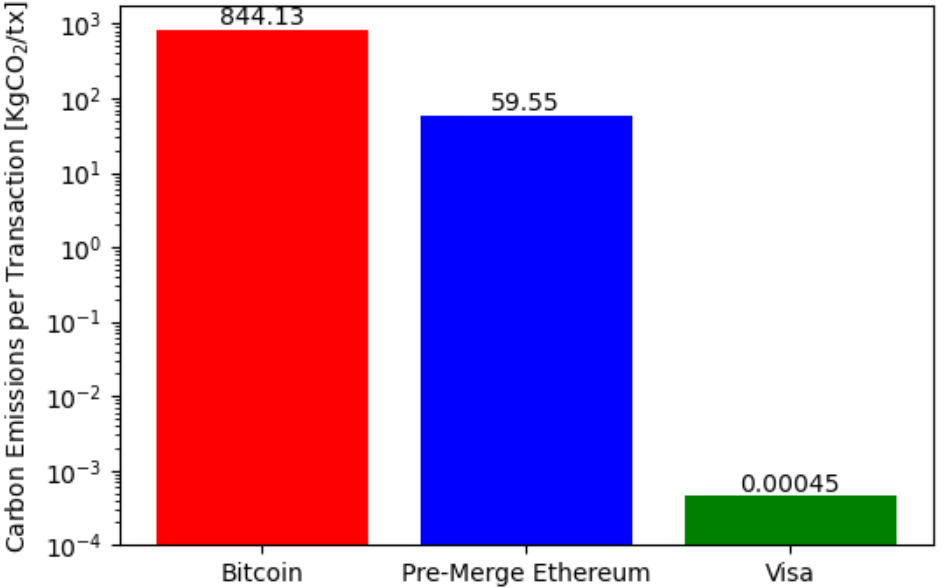
\includegraphics[width=13cm,center]{Figures/CarbonEmissionsPlot.png}
    \caption{Carbon emissions per transaction for Bitcoin, Ethereum 1.0 and Visa plotted on a logarithmic scale. The code is in Appendix C, \fref{Figure:CarbonEmissionsPlotCode}. Data source: \cite{Kohli2023AnSolutions} }
    \label{Figure:CarbonEmissionsPlot}
\end{figure}

The stark difference in emissions per transaction is highlighted in \fref{Figure:CarbonEmissionsPlot}, especially due to using a logarithmic scale. These carbon emissions can be used as a proxy of environmental damage \cite{2022VisaReport}. This environmental damage linked to energy consumption renders it highly unsustainable.

Apart from cryptocurrencies, blockchain technology is increasingly being employed to track provenance in supply chains, especially drug-supply chains \cite{Labaran2021TheNigeria}. The literature contains numerous examples of such implementations using blockchain found in \tref{Table:DrugSupplyImplementations}, with some claiming to be low-energy solutions employing off-chain storage and non-PoW consensus mechanisms.

\begin{table}[!htb]
\centering
\begin{tabular}{|l"l|l|l|l|l|}
\hline
\textbf{Topic} &
  \textbf{\begin{tabular}[c]{@{}l@{}}Vaccine \\ Delivery \\ Solution\end{tabular}} &
  \textbf{\begin{tabular}[c]{@{}l@{}}Medication \\ Anti-fraud \&\\ Traceability\end{tabular}} &
  \textbf{\begin{tabular}[c]{@{}l@{}}‘Everyware’\\ Platform\end{tabular}} &
  \textbf{\begin{tabular}[c]{@{}l@{}}Analysis of \\ Blockchain in \\ Healthcare\end{tabular}} &
  \textbf{\begin{tabular}[c]{@{}l@{}}Drug \\ Traceability\\ Solution\end{tabular}} \\ \thickhline
\textbf{\begin{tabular}[c]{@{}l@{}}Blockchain \\ Platform\end{tabular}} &
  Ethereum &
  Ethereum &
  Hedera &
  \begin{tabular}[c]{@{}l@{}}Hyperledger\\ Fabric\end{tabular} &
  Ethereum \\ \hline
\textbf{\begin{tabular}[c]{@{}l@{}}Consensus \\ Algorithm\end{tabular}} &
  PoW &
  \begin{tabular}[c]{@{}l@{}}practical\\ Byzantine\\ fault tolerance\end{tabular} &
  \begin{tabular}[c]{@{}l@{}}Hashgraph\\ Consensus\end{tabular} &
  \begin{tabular}[c]{@{}l@{}}Redundant\\ Byzantine \\ fault tolerance\end{tabular} &
  PoW \\ \hline
\textbf{\begin{tabular}[c]{@{}l@{}}Type of \\ Operations\end{tabular}} &
  \begin{tabular}[c]{@{}l@{}}Public   \\ Permissioned\end{tabular} &
  \begin{tabular}[c]{@{}l@{}}Public   \\ Permissioned\end{tabular} &
  \begin{tabular}[c]{@{}l@{}}Public \\ Permissioned\end{tabular} &
  \begin{tabular}[c]{@{}l@{}}Private   \\ Permissioned\end{tabular} &
  \begin{tabular}[c]{@{}l@{}}Public\\ Permissioned\end{tabular} \\ \hline
\textbf{Currency} &
  Ether &
  None &
  None &
  None &
  Ether \\ \hline
\textbf{\begin{tabular}[c]{@{}l@{}}Off-chain \\ storage\end{tabular}} &
  Yes &
  None &
  Yes &
  None &
  Yes \\ \hline
\textbf{\begin{tabular}[c]{@{}l@{}}Customisable \\ Component\end{tabular}} &
  \begin{tabular}[c]{@{}l@{}}Ethereum\\ Smart \\ Contracts\end{tabular} &
  \begin{tabular}[c]{@{}l@{}}Ethereum\\ Smart\\ Contracts\end{tabular} &
  Yes &
  \begin{tabular}[c]{@{}l@{}}Docker\\ Container\end{tabular} &
  \begin{tabular}[c]{@{}l@{}}Ethereum\\ Smart \\ Contracts\end{tabular} \\ \hline
\textbf{\begin{tabular}[c]{@{}l@{}}Energy \\ Consumption\end{tabular}} &
  High &
  Low &
  Very Low &
  Low &
  High \\ \hline
\textbf{Source} &
  \cite{Musamih2021Blockchain-BasedVaccines} &
  \cite{Zhu2020ATraceability} &
  \cite{Platform}, \cite{TechnologyLtd} &
  \cite{Mettler2016BlockchainHere} &
  \cite{Musamih2021AChain} \\ \hline
\end{tabular}
\caption{Several implementations of drug-supply chain solutions that use blockchain technology, with 3 implementations using Ethereum 1.0}
\label{Table:DrugSupplyImplementations}
\end{table}

However, newly established independent blockchains, whether intended for cryptocurrency or provenance purposes, often struggle to maintain the two primary benefits of blockchain technology, either through security breaches due to a lack of users or centralization through permissioned blockchain solutions. 51\% attacks occur when a malicious miner or group controls over 50\% of a network's computational power. Small blockchains with few participants are more vulnerable as it is easier for a malicious actor to acquire the necessary computational power, leaving the blockchain susceptible to tampering and theft \cite{Redman2021PrivacyErased}.









% _______________________________________________________________
% -_____________________________________________________________________________

% __________________________________________________________________________________________-
% -_____________________________________________________________________________

\subsection{Mathematical Modelling}
\label{MathematicalModellingLitRev}

Modelling is about making some assumptions in order to simplify a complex system and test a hypothesis. There are a number of approaches for scientific model building, descriptive and rule-based modelling \cite{SayamaINTRODUCTIONSYSTEMS}. This paper employs the latter.

\textbf{Rule-based modelling} involves coming up with certain dynamic rules and limitations that can explain the behaviour of a system. It is all about capturing how the model will behave over time, usually done using quantitative methods.

Observations must be turned into mathematical equations, but this can be challenging as the system's unique properties may be ones we are not familiar with (for example, large networks and nonlinearity). A book on modelling complex systems claims the 4 things to keep in mind when modelling include \cite{SayamaINTRODUCTIONSYSTEMS}:

\begin{itemize}
    \item The key research questions that need to be addressed
    \item To answer the research questions, what scale is most appropriate to describe the systems, microscopic or macroscopic
    \item How the system is structured
    \item What are all the possible states of the system, and how it changes over time
\end{itemize}

This study uses the microscopic details of the Ethereum protocol (how attestations are handled) to model its macroscopic effects at scale (increase in overall energy usage). 



% ____________________________________________________________________---

% ______________________________________________________________________________
% -_____________________________________________________________________________

% __________________________________________________________________________________________-


\section{Modelling PoW Energy Consumption}

This section aims to analyse a wide range of papers on the topic of electricity consumption of blockchain. The steps for a structured literature review laid out by \cite{Crosby2015BlockChainBitcoin} are loosely followed. 

Most papers in this niche field of research emphasise Bitcoin and PoW cryptocurrencies. It shows a clear gap in the literature for more work to be done on modelling the electricity consumption of non-PoW blockchains, as this study intends to do.
% -_____________________________________________________________________________

Paper \cite{Sedlmeir2020TheMyth} attributes almost all the energy consumed by PoW blockchains to the PoW consensus mechanism alone. The other factors contribute a negligible amount of electricity in comparison. However, estimating the electricity consumption of blockchain consensus mechanisms can be challenging due to the scarcity of accurate information on the number of network participants and their hardware configurations. The same study also confirms that Proof-of-Work (PoW) blockchains consume a disproportionate amount of electricity relative to the actual utility they offer. When comparing PoW electricity estimates to those of non-PoW blockchains, the results were several orders of magnitude lower for non-PoW blockchains \cite{Sedlmeir2020TheMyth}. Due to non-PoW consensus algorithms having such a small energy footprint, the energy consumption of a non-PoW blockchain cannot solely be attributed to its consensus algorithm but also to a range of other factors that come with having a large decentralised network. Studies in this area are sparse and are discussed in section ****. 

\begin{figure}[h]
    \centering
    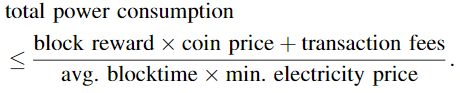
\includegraphics[width=8cm,center]{Figures/SimplePoWModel.png}
    \caption{A simple model estimating the upper bound of electricity consumption of a PoW blockchain \fref{Figure:CarbonEmissionsPlotCode}. Source: \cite{Sedlmeir2020TheMyth} }
    \label{Figure:SimplePoWModel}
\end{figure}

Energy consumption in many PoW-focused papers is attributed to metrics like block rewards, coin price, transaction fee, average block time and hashing difficulty which are all publicly available and reliable metrics, \cite{Mcdonald2022EthereumEstimate}. Such a model is shown in \fref{Figure:SimplePoWModel}.

% -_____________________________________________________________________________
Another data-driven study collected and analysed publicly available data to derive a joule per hash (per 'nonce' value calculated) value based on a small number of direct measurements from a small testbed network \cite{Cole2018ModelingAlgorithms}. Using a LASSO (Least Absolute Shrinkage and Selection Operator) regression model, the researchers were able to estimate the energy usage of PoW cryptocurrencies with 92\% accuracy. The same cannot be done for PoS blockchains due to the lack of data availability and the vast range of factors affecting its energy consumption outside of the consensus protocol itself.

Digiconomist \cite{BitcoinDigiconomist} and CBECI \cite{CambridgeCBECI} are two well-known real-time models used to estimate the energy consumption of Bitcoin. These are highly credible models and have been referenced many times in the wider literature, such as \cite{Cole2018ModelingAlgorithms}, \cite{Lei2021BestRecommendations}, and \cite{Erdogan2022AnalyzingSustainability}, \cite{Platt2022TheProof-of-Work}, respectively. Both models use live tracking of Bitcoin's price and mining hash rate to maintain accuracy but take different approaches to arrive at similar estimates. Digiconomist's top-down approach estimates the total revenue earned by USA-based Bitcoin miners. It assumes that 60\% of this revenue is spent on operational costs, primarily electricity, in the case of PoW. By using the global average electricity costs, the model is able to calculate Bitcoin's energy consumption. In contrast, CBECI uses a bottom-up approach, focusing on selecting contemporary mining equipment that maximises the number of hashes computed per Joule of energy used. The model then uses a profitability threshold to extrapolate Bitcoin's annual electricity consumption. This paper takes inspiration from both approaches introduced by these models to develop a model for non-PoW blockchains.





% __________________________________________________________________________________________-
% __________________________________________________________________________________________-


\subsection{ Electricity Consumption of PoS Blockchains }
\label{LitRevExistingModels}

There is a large gap in the literature on this niche field of research. This section analyses the work done in this area and why it needs to be improved upon.

A study by Powell et al., aimed at making recommendations for building greener blockchains, suggested a simple formula to calculate the energy of the Polkadot blockchain that employs PoS consensus \cite{Powell2021AWARENESSBLOCKCHAIN}. Their model was the first of its kind, and it follows: 
\begin{align}
   \boldsymbol{\mathrm{\text{Polkadot Energy Consumption } = }}
   &\boldsymbol{\mathrm{\text{ Energy per server }* \text{ number of servers } } } \nonumber\\
   &\boldsymbol{\mathrm{* \text{ 24 hours } *\text{ 365 days }}} \nonumber
\end{align}

A recent study by UCL Centre for Blockchain Technologies \cite{PlattDiscussionProof-of-Work} built upon this equation by establishing a mathematical relationship between validator number, network load and hardware configuration to estimate the energy consumption of the PoS consensus protocol in isolation. Their approach was to build upon past literature using new data sets from various sources, including empirical data from CCRI report \cite{CryptoCarbonRatingsInstitute2022TheNetwork} and other publicly available metrics while avoiding time-consuming first-hand experimentation, just like this study aims to do. 

\begin{align}
   \boldsymbol{\mathrm{\text{Energy Per Transaction} = }}
   &\boldsymbol{\mathrm{\frac{\text{ Energy per Validator }* \text{ Number of Validators } }{\text{ Number of Transactions }}} } \nonumber\\ \nonumber
\end{align}

Their generalised model performs well for a few different PoS blockchains, with Ethereum being one of them. In fact, R3, a private company that run the Corda blockchain have also used the same equation to estimate its energy consumption \cite{JustBlog}. However, amidst this generalisation, the UCL study makes a critical mistake of not differentiating between validators (currently $\sim$500,000 \cite{EthereumEthereum.orgc}) and Full Nodes ($\sim$15,000 \cite{NodewatchAnalytics}). Their model only considers validators and estimates only the PoS consensus protocol’s energy usage in isolation. Thus, incomplete in its calculation of network-wide energy consumption by ignoring factors such as the 'Full Nodes' that aren't actively participating in forming consensus but greatly contribute to securing the blockchain. Such factors have not been ignored in the model proposed by this study. The UCL study also relies on speculative assumptions as it was written before Ethereum’s upgrade to PoS consensus (now the world’s largest PoS blockchain). Hence, the most significant PoS blockchain was not included in its study.

The future work mentioned in the study is closely aligned with the focus of this study, which aims to build a more comprehensive model by incorporating additional factors and considering different node types.


\textbf{The CCRI Study } 
\label{CCRIModelLitRev}
The state-of-the-art research conducted by Crypto Carbon Ratings Institute focuses specifically on the electricity consumption of post-merge PoS Ethereum. It provided the most up-to-date empirical data that has been cited in other studies such as this one \cite{CryptoCarbonRatingsInstitute2022TheNetwork}. These researchers decided on 6 commodity hardware configurations that they ran idly for base power consumption figures and then ran each major EL and CL client software separately, taking 48-hour electricity measurements. The data was used in their equation (detailed in \sref{CCRIBaseEqnSection}), which was formulated using a combination of experimentation and prior domain knowledge. The accuracy of the model was confirmed by comparing the actual measurements from running Full Nodes to their estimated values, which were found to be highly precise.

Assumptions and shortcomings of this study:
\begin{enumerate}
    \item Different combinations of clients were run to form Full Nodes. However, the next step of running a validator client on the Full Node was not taken due to the barrier of staking 32 ETH. The effects of running a validator client on top of a Full Node were assumed to be negligible.
    
    \item The synchronisation energy consumed whilst bootstrapping Full Nodes was not considered.
    
    \item Other node types, such as Light and Archive Nodes, were not considered, presumably due to assuming that they would have negligible effects.

    \item The electricity data was collected using computer software, but there is no information available on the type of power supply and mainboard used in the experiments. Therefore, the measurements only account for the electricity consumed by the computer itself and do not factor in the power draw 'At-Wall' or any electrical inefficiencies. \cite{Warkozek2012ACenters}
\end{enumerate}
 


% -_____________________________________________________________________________


% Quick intro on AVX operations, what is TDP and why that is the upper limit of CPU power consumption
% AVX instructions enable the processor to perform multiple floating-point operations at the same time, resulting in faster computation and improved performance. \cite{Schuchart2016TheScale}

% ______________________________________________________________________________
% -_____________________________________________________________________________

% __________________________________________________________________________________________-

% \section{Key Points Covered}
